\section{Plasma-Wakefield Cold-Linear Closed Form --- Full Data Record}
\label{app:wakefield}

This appendix is the full data record for the cold-linear
plasma-wakefield kernel (pipeline stages
\textcircled{\scriptsize 2}\textcircled{\scriptsize 3},
\S\ref{sec:plasma}). It states the Dawson plasma-frequency,
plasma-wavelength, and cold non-relativistic wave-breaking-field
relations, the representative gas-jet density operating point, the
selftest 5/5 GREEN result, and the two \tierGreen\ verify atoms
(\verb|wakefield_e0_gv_m|, \verb|wakefield_lambda_um|) landed in
hexa-lang PR~\#1007. Every digit traces to
\texttt{companion/verify-ledger.json}.

% -------------------------------------------------------------------------
\subsection{The three cold-linear relations}
\label{app:wf-eq}

In the cold, linear (small-amplitude) limit a relativistic drive
displaces plasma electrons against the immobile ion background, exciting
a Langmuir wave. Three standard closed forms
\citep{dawson1959,esarey2009lpa} fix the wakefield:
\begin{align}
\omega_p &= \sqrt{\frac{n_e\,e^{2}}{\varepsilon_0\,m_e}}
   && \text{(plasma angular frequency)}, \label{eq:app-wp}\\[2pt]
\lambda_p &= \frac{2\pi c}{\omega_p}
   && \text{(plasma wavelength)}, \label{eq:app-lam}\\[2pt]
E_0 &= \frac{m_e c\,\omega_p}{e}
   = \frac{c}{e}\sqrt{\frac{n_e m_e}{\varepsilon_0}}
   && \text{(cold non-rel.\ wave-breaking, Dawson)}. \label{eq:app-e0}
\end{align}
The kernel (\verb|stdlib/cern/plasma_wakefield.hexa|) evaluates
\eqref{eq:app-wp}--\eqref{eq:app-e0} from CODATA constants
($e=\SI{1.602176634e-19}{C}$, $\varepsilon_0=\SI{8.8541878128e-12}{F/m}$,
$m_e=\SI{9.1093837015e-31}{kg}$, $c=\SI{299792458}{m/s}$), taking the
density input in \si{cm^{-3}} (the LWFA-literature unit) and converting
to \si{m^{-3}} internally.

\paragraph{Engineering coefficients.} Folding the constants gives the
forms quoted across the LWFA literature, which the selftest cross-checks:
\begin{equation}
E_0\,[\si{V/m}] \approx 96\,\sqrt{n_e\,[\si{cm^{-3}}]},
\qquad
\lambda_p\,[\si{\micro\meter}] \approx
   \frac{3.34\times 10^{10}}{\sqrt{n_e\,[\si{cm^{-3}}]}}.
\label{eq:app-coeff}
\end{equation}

% -------------------------------------------------------------------------
\subsection{Deriving the engineering coefficients}
\label{app:wf-coeff}

The two literature coefficients in Eq.~\ref{eq:app-coeff} fall directly
out of the constants. Folding $\omega_p = \sqrt{n_e e^2/(\varepsilon_0
m_e)}$ into $E_0 = m_e c\,\omega_p/e = c\sqrt{n_e m_e/\varepsilon_0}$ and
evaluating at $n_e = \SI{1}{cm^{-3}} = \SI{e6}{m^{-3}}$ gives the
per-$\sqrt{n_e}$ coefficient
\begin{equation}
\frac{E_0}{\sqrt{n_e\,[\si{cm^{-3}}]}}
  = c\sqrt{\frac{\SI{e6}{}\,m_e}{\varepsilon_0}}
  = \SI{96.159}{V/m},
\end{equation}
matching the textbook $\approx\!96$ to $0.2\%$. Likewise
$\lambda_p = 2\pi c/\omega_p$ scales as $1/\sqrt{n_e}$, and at
$n_e=\SI{1}{cm^{-3}}$ the product
\begin{equation}
\lambda_p\,[\si{\micro\meter}]\cdot\sqrt{n_e\,[\si{cm^{-3}}]}
  = \SI{3.3389e10}{},
\end{equation}
matching the textbook $\approx\!\num{3.34e10}$ to $0.05\%$. Both
coefficients are verified by the selftest cross-checks
(\S\ref{app:wf-selftest}); they are not free parameters but consequences
of the closed form.

% -------------------------------------------------------------------------
\subsection{Density-to-gradient scaling}
\label{app:wf-scaling}

Table~\ref{tab:app-wf} and Figure~\ref{fig:wakefield} give the kernel's
density sweep over $n_e = 10^{16}$--$10^{19}\,\si{cm^{-3}}$. The
operating point $n_e=10^{18}\,\si{cm^{-3}}$ (typical LWFA gas-jet) yields
$E_0 = \SI{96.16}{GV/m}$ --- three to four orders of magnitude above the
$\sim$\,tens-of-\si{MV/m} of an RF cavity, which is the entire motivation
for the tabletop regime --- and $\lambda_p = \SI{33.39}{\micro\meter}$.

\begin{table}[h]
\centering
\small
\setlength{\tabcolsep}{6pt}
\begin{tabular}{@{}l c c@{}}
\toprule
$n_e$ (cm$^{-3}$) & $E_0$ (GV/m) & $\lambda_p$ ($\mu$m) \\
\midrule
$10^{16}$            & 9.6159   & 333.894 \\
$3\times 10^{16}$    & 16.6553  & 192.774 \\
$10^{17}$            & 30.4082  & 105.587 \\
$3\times 10^{17}$    & 52.6686  & 60.961  \\
$\mathbf{10^{18}}$   & \textbf{96.1592} & \textbf{33.3894} \\
$3\times 10^{18}$    & 166.5526 & 19.277  \\
$10^{19}$            & 304.0821 & 10.5587 \\
\bottomrule
\end{tabular}
\caption{Cold-linear wakefield scalings from
\texttt{plasma\_wakefield.hexa}. The bold $10^{18}\,\si{cm^{-3}}$ row is
the verify-ledger operating point. $E_0\propto\sqrt{n_e}$ and
$\lambda_p\propto 1/\sqrt{n_e}$ per Eqs.~\ref{eq:app-wp}--\ref{eq:app-e0}.}
\label{tab:app-wf}
\end{table}

\begin{figure}[h]
\centering
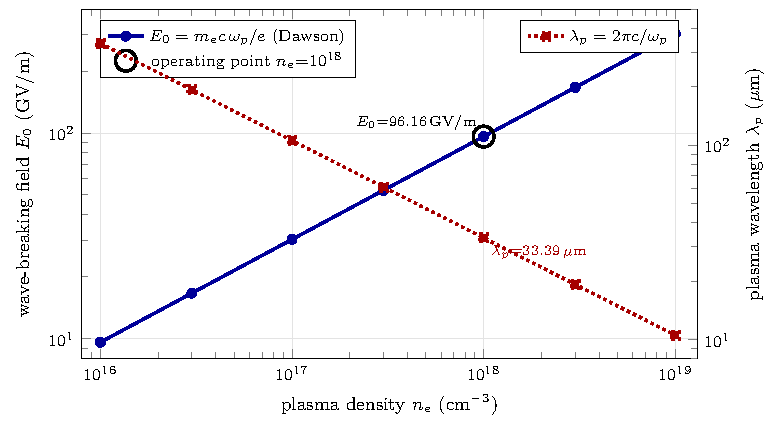
\includegraphics[width=0.9\linewidth]{figures/fig05_wakefield_density.pdf}
\caption{Wave-breaking field $E_0$ (left, blue) and plasma wavelength
$\lambda_p$ (right, red) versus plasma density $n_e$, on log--log axes.
The black-ringed marker is the $n_e=10^{18}\,\si{cm^{-3}}$ operating
point ($E_0=\SI{96.16}{GV/m}$, $\lambda_p=\SI{33.39}{\micro\meter}$),
the two values registered as \tierGreen\ verify atoms. $E_0$ rises and
$\lambda_p$ falls as $\sqrt{n_e}$; the GV/m gradient is the tabletop
advantage over RF.}
\label{fig:wakefield}
\end{figure}

% -------------------------------------------------------------------------
\subsection{Worked evaluation (the $10^{18}$ operating point)}
\label{app:wf-worked}

The three closed forms evaluated at the anchor density
$n_e = \SI{e18}{cm^{-3}} = \SI{e24}{m^{-3}}$ trace as follows. The plasma
angular frequency (Eq.~\ref{eq:app-wp}) is
\begin{equation}
\omega_p = \sqrt{\frac{\SI{e24}{}\,(\num{1.602177e-19})^2}
   {(\num{8.854188e-12})(\num{9.109384e-31})}}
   = \SI{5.6414602e13}{rad/s},
\end{equation}
from which the wavelength (Eq.~\ref{eq:app-lam}) is
\begin{equation}
\lambda_p = \frac{2\pi c}{\omega_p}
   = \frac{2\pi\,(\num{2.99792458e8})}{\num{5.6414602e13}}
   = \SI{3.338943e-5}{m} = \SI{33.38943}{\micro\meter},
\end{equation}
and the Dawson wave-breaking field (Eq.~\ref{eq:app-e0}) is
\begin{equation}
E_0 = \frac{m_e c\,\omega_p}{e}
   = \frac{(\num{9.109384e-31})(\num{2.99792458e8})(\num{5.6414602e13})}
   {\num{1.602177e-19}}
   = \SI{96.15920}{GV/m}.
\end{equation}
These are the exact \tierGreen\ atom values (\S\ref{app:wf-selftest}),
reproduced from CODATA constants with no fitting.

% -------------------------------------------------------------------------
\subsection{Selftest (5/5 GREEN) and the two atoms}
\label{app:wf-selftest}

The kernel's selftest pins three value anchors at
$n_e=10^{18}\,\si{cm^{-3}}$ and two literature engineering-coefficient
cross-checks, all to a relative tolerance of $10^{-6}$ on the value pins
and $5\times 10^{-3}$ on the coefficients:

\begin{table}[h]
\centering
\small
\setlength{\tabcolsep}{5pt}
\begin{tabular}{@{}l c c c@{}}
\toprule
check & value & reference & status \\
\midrule
$\omega_p$ @ $10^{18}$ (rad/s)        & \num{5.6414602e13} & \num{5.6414602e13} & PASS \\
$\lambda_p$ @ $10^{18}$ ($\mu$m)      & 33.3894327 & 33.3894327 & PASS \\
$E_0$ @ $10^{18}$ (GV/m)              & 96.1591987 & 96.1591987 & PASS \\
coeff $E_0/\sqrt{n_e}$ (V/m)          & 96.159     & 96.0       & PASS ($<0.2\%$) \\
coeff $\lambda_p\sqrt{n_e}$ ($\mu$m)  & \num{3.339e10} & \num{3.34e10} & PASS ($<0.05\%$) \\
\bottomrule
\end{tabular}
\caption{The \texttt{plasma\_wakefield.hexa} selftest (5/5 GREEN). The
first three are float64 value pins (independent closed-form recompute);
the last two confirm the kernel reproduces the LWFA-literature
engineering coefficients of Eq.~\ref{eq:app-coeff}.}
\label{tab:app-wf-selftest}
\end{table}

Two of these graduate to registered verify atoms (hexa-lang PR~\#1007),
reproduced verbatim from the ledger:

\begin{lstlisting}
fn       : wakefield_e0_gv_m        args : [n_e=1e18 cm^-3]
expected : 96.15919872735485   observed : 96.15919872735485   |delta| : 0.0
tier     : SUPPORTED-NUMERICAL                              PR : #1007  stage : 3

fn       : wakefield_lambda_um      args : [n_e=1e18 cm^-3]
expected : 33.38943270215429   observed : 33.38943270215429   |delta| : 0.0
tier     : SUPPORTED-NUMERICAL                              PR : #1007  stage : 2
\end{lstlisting}

% -------------------------------------------------------------------------
\subsection{Honest scope --- cold and linear}
\label{app:wf-honesty}

\noindent\fbox{\parbox{0.97\linewidth}{\small\textbf{Honest scope.} The
kernel is \emph{cold linear theory only}. It omits the relativistic
wave-breaking boost (the Akhiezer--Polovin factor
$\sqrt{2(\gamma_p-1)}$), the laser/beam-driver envelope, the dephasing
length, pump depletion, beam loading, ion motion, and all 2-D/3-D
geometry. The \tierGreen\ verdict certifies the leading-order closed form
is reproduced; it is the \emph{validating reference} that the 1-D linear
PIC parity (Appendix~\ref{app:pic}) is checked against. The nonlinear
blowout (bubble) regime, where $E_0$ is boosted and the wave shape
departs from the cold-linear form, is a GPU-heavy downstream item
(Appendix~\ref{app:downstream}) and is not claimed here.}}
